\subtop{Schranken für die Winkelauflösung in geradlinigen Layouts}{-1.725}
\begin{itemize}[itemsep=-1pt]
	\item gesucht ist eine geradlinige Einbettung von einem planaren Graphen $G$ mit maximalem
		\[x_{min}=\min\limits_{\substack{v\in V,~f\in \mathcal{F}\\v\text{ inzident zu }f}}\{x(v,f)\}\]
	\item $\mathcal{NP}$-schwer
\end{itemize}
\begin{description}[itemsep=-1pt]
	\item[Einschränkung:] planare kombinatorische Einbettung ist gegeben
	\item[Modell:] Formulierung des Problems als Flussmodell (liefert untere Schranke für $x_min$)
\end{description}
\subsection{Grundidee der Konstruktion}
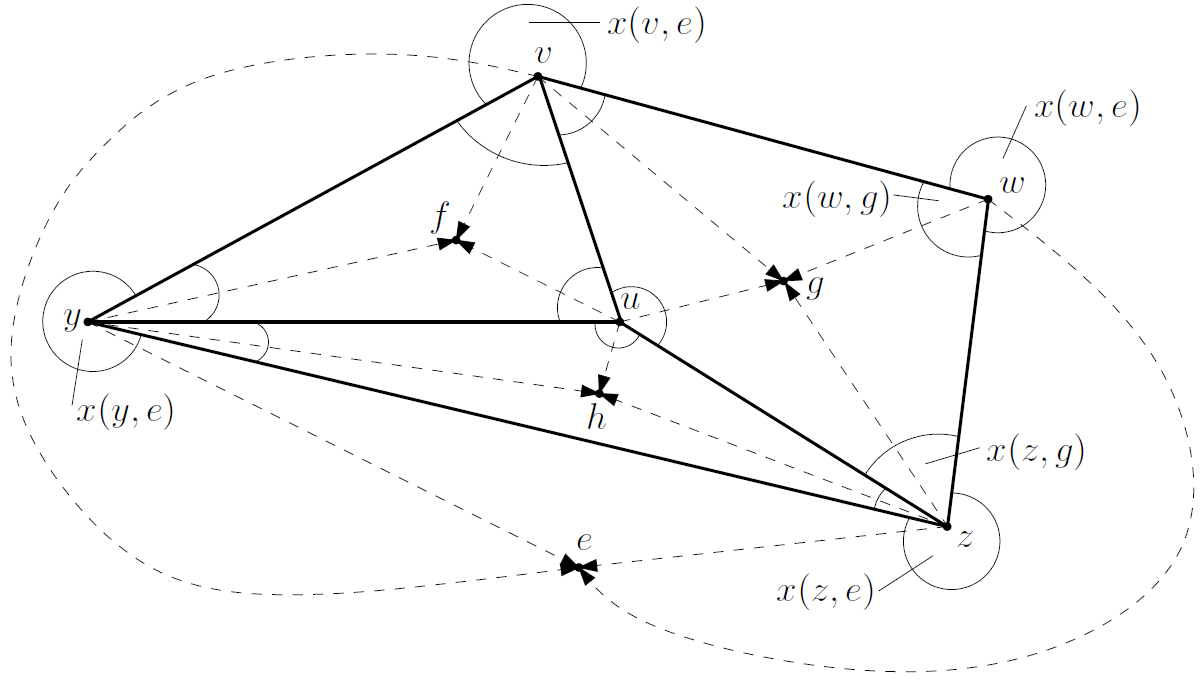
\includegraphics[width=0.8\textwidth]{Pics/3_construction.png}\\
\textbf{Es gilt:}
\begin{description}[itemsep=-1pt]
	\item[1. Knotenbedingung:] $\forall v\in V~:~\sum\limits_{f\in \mathcal{F}\text{ inzident zu }v}x(v,f)=2\cdot\pi$
	\item[2. Facettenbedingung:] 
		\begin{eqnarray*}
			\forall f\in \mathcal{F}\setminus\{f_0\}~:&\sum\limits_{v\in \text{ inzident zu }f}x(v,f)&=(d_G(f)-2)\cdot\pi\\
			f_0~:&\sum\limits_{v\in \text{ inzident zu }f_0}x(v,f_0)&=d_G(f_0)\cdot\pi-(d_G(f_0)-2)\cdot\pi\\
			&&=(d_G(f_0)+2)\cdot \pi
		\end{eqnarray*}
\end{description}
\topbreak
\vspace*{-2\baselineskip}
\subsection{Definition des Flussnetzwerks $N(G)=(D=(W,A),b,l,u)$}
\vspace*{-\baselineskip}
\begin{eqnarray*}
	W&=&V\cup \mathcal{F}\\
	A&=&\{(v,f)\in V\times \mathcal{F}, v\text{ inzident zu }f\}\\
	b(v)&=&2\pi,~\forall v\in V\\
	b(f)&=&-(d_G(f)-2)\pi,~\forall f\in\mathcal{F}\setminus\{f_0\}\\
	b(f_0)&=&-(d_G(f)+2)\pi\\
	l(a)&=&0,~\forall a\in A\\
	u(a)&=&2\pi,~\forall a\in A
\end{eqnarray*}
\subsection{Definition des Flussnetzwerks $N_{s,t}(G)=(D=(W_{s,t},A_{s,t}),l,u)$}
\vspace*{-\baselineskip}
\begin{eqnarray*}
	W_{s,t}&=&W\cup \{s,t\}\\
	A_{s,t}&=&A\cup \{(s,v)|v\in V\}\cup \{(f,t)|f\in \mathcal{F}\}\\
	l(s,v)&=&l(f,t)=0,~~~\forall v\in V,~f\in\mathcal{F}\\
	u(s,v)&=&2\pi,~\forall v\in V\\
	u(f,t)&=&-(d_G(f)-2)\pi,~~~\forall f\in\mathcal{F}\setminus\{f_0\}\\
	u(f_0,t)&=&-(d_G(f)+2)\pi
\end{eqnarray*}
\subsection{untere Schranke von $x_{min}$}
\vspace*{-0.5\baselineskip}
$\alpha$ ist genau dann eine untere Schranke von $x_min$ für einen maximalen Fluss $x$, falls $\max w(x_{s,t})$ von $N_{s,t}(G)$ gleich $\max w(x'_{s,t})$ von $N'_{s,t}(G) = ((W_{s,t},A_{s,t}),l',u)$ mit $l'(a)=\alpha,~\forall a\in A$\\
$\Rightarrow$ Beweis mit Ford und Fulkerson (Kapazität jedes $s$-$t$-Schnittes in $N'_{s,t}(G)$ ist nicht kleiner als due Kapazität eines minimalen $s$-$t$-Schnittes in $N_{s,t}(G)$).

\subsection{Konstruktion eines Flusses}
\begin{minipage}{0.4\textwidth}
	\usetikzlibrary{positioning,patterns,calc,arrows}

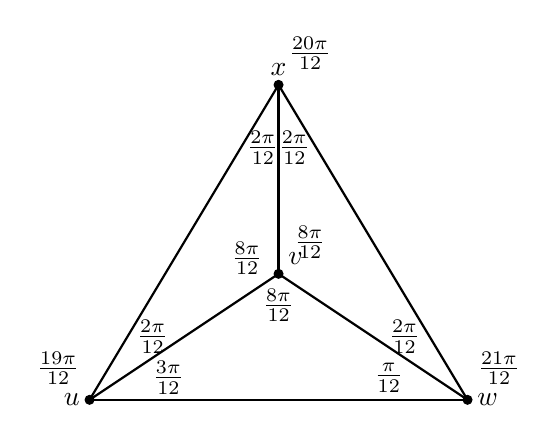
\begin{tikzpicture}[scale=0.8]
\def\tw#1{$\frac{#1\pi}{12}$}

\coordinate[label={10:$v$}](1) at (0,0);
\coordinate[label={90:$x$}](2) at (0,3);
\coordinate[label={180:$u$}](3) at (-3,-2);
\coordinate[label={0:$w$}](4) at (3,-2);

\foreach \x in {1,...,4}{
	\draw[fill](\x)circle[radius=2pt];
}
\foreach \x in {1,...,3}{
	\foreach \y in {\x,...,4}
		\draw[-,thick](\x)--(\y);
}

\foreach \x/\y/\v in {}
	\node at (\x,\y) {\tw{\v}};

\foreach \x/\y/\v in {0.5/3.5/20,-3.5/-1.5/19,3.5/-1.5/21,-2/-1/2,-1.75/-1.65/3,-0.25/2/2,0.25/2/2,2/-1/2,1.75/-1.65/,0/-0.5/8,-0.5/0.25/8,0.5/0.5/8}
	\node at (\x,\y) {\tw{\v}};

\end{tikzpicture}
\end{minipage}
\begin{minipage}{0.55\textwidth}
	\subsubsection{Definition}
	\begin{description}[itemsep=-1pt]
		\item[lokal konstistent:] Zuweisung von Winkelwerten, die Knoten- und Facettenbedingungen erfüllen\\
		\item[\textbf{\color{red}\Large !}] nicht zu jeder lokal konsistenten Zuweisung gibt es auch eine Einbettung, die diese realisiert
	\end{description}
\end{minipage}\\
\example{Konstruktion}{
	\ \\
	\begin{minipage}{0.35\textwidth}
		\usetikzlibrary{positioning,patterns,calc,arrows}

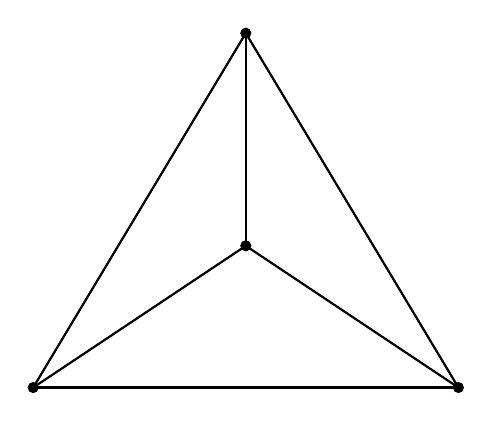
\begin{tikzpicture}[scale=0.9]
\def\tw#1{$\frac{#1\pi}{12}$}

\coordinate(1) at (0,0);
\coordinate(2) at (0,3);
\coordinate(3) at (-3,-2);
\coordinate(4) at (3,-2);

\foreach \x in {1,...,4}{
	\draw[fill](\x)circle[radius=2pt];
}
\foreach \x in {1,...,3}{
	\foreach \y in {\x,...,4}
		\draw[-,thick](\x)--(\y);
}

\foreach \x/\y/\v in {}
	\node at (\x,\y) {\tw{\v}};


\end{tikzpicture}
	\end{minipage}
	$\Longrightarrow$
	\begin{minipage}{0.55\textwidth}
		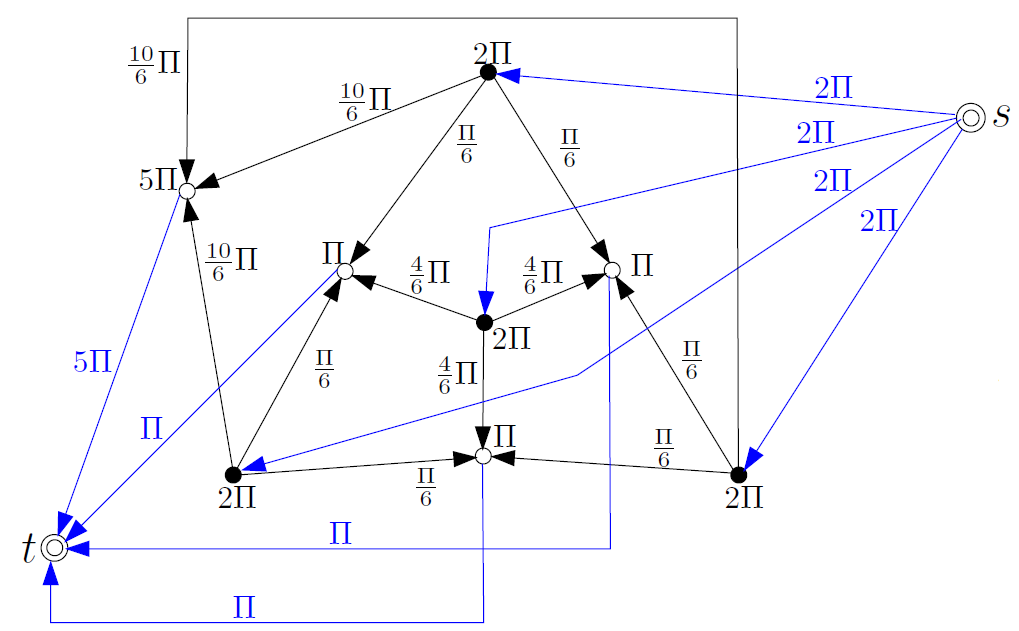
\includegraphics[width=\textwidth]{Pics/3_construction-2.png}\\
		Fluss $x$ in $N'_{s,t}(G)$ mit $w(x)=8\pi$ (maximal)\\
		$x_{min}=\frac{\pi}{6}$
	\end{minipage}
}
\topbreak
\vspace*{-2\baselineskip}
\begin{itemize}[itemsep=-1pt]
	\item es gibt für jeden triangulierten, planar eingebetteten Graphen eine lokal konsistente Winkelzuweisung mit $x_{min}\in\Omega(\dfrac{1}{\Delta_G})$
	\item oberes liefert nur eine obere Schranke für die untere Schranke, da nicht jede lokal konsistente Zuweisung realisierbar ist
	\item ein \textbf{Dreiecksgraph} ist bis auf die äußere Facette trianguliert (z.B. der Wheel-Graph ($W_d$))
	\item für jeden planaren Dreiecksgraphen mit kombinatorischer Einbettung, beschrieben durch $\mathcal{F}$, und einer vorgegebenen Winkelzuweisung ($\alpha_i,\beta_i,\gamma_i,~\forall 1\leq i\leq d$) gibt es eine geradlinige Realisierung der Einbettung mit dieser Winkelzuweisung, gdw.
		\begin{enumerate}[itemsep=-1pt]
			\item $\sum\limits_{i=0}^{d}\gamma_i=2\pi,~\forall 1\leq i\leq d$
			\item $\alpha_i+\beta_i+\gamma_i=\pi,~\forall 1\leq i\leq d$
			\item $\prod\limits_{i=0}^{d}\dfrac{\sin\alpha_i}{\sin\beta_i}=1$
		\end{enumerate}
	\vspace*{-\baselineskip}
	\ProofOne{$\Rightarrow$}
	\vspace*{-0.5\baselineskip}
	\begin{enumerate}[itemsep=-1pt]
		\item[1./2.] gilt durch Definition
		\item[3.] $L_i$ ist die Länge bei Kante $e_i$ zwischen den Winkeln $\beta_i$ und $\alpha_{(i\mod d)+1}$\\
		$\Rightarrow \prod\limits_{i=0}^{d}\dfrac{L_{(i\mod d)+1}}{L_i}=\dfrac{L_2}{L_1}\cdot \dfrac{L_3}{L_2}\cdot \ldots\cdot \dfrac{L_1}{L_d}=1$\\
		$\Rightarrow \dfrac{L_{(i\mod d)+1}}{L_i}=\dfrac{\sin \alpha_{(i\mod d)+1}}{\sin \beta_{(i\mod d)+1}}$\\
		$\Rightarrow$ Bedingung 2 ist wahr
	\end{enumerate}
	\vspace*{-\baselineskip}
	\ProofOne{$\Leftarrow$ (Konstruktion der Zeichnung mit den Winkeln)}
	\vspace*{-0.5\baselineskip}
	\begin{itemize}[itemsep=-1pt]
		\item beliebiges $L_1$ wählen, Zeichnen der Kante $\{v,v_2\}$
		\item Berechnen von $L_{i+1}$ mit $L_i~~(i=1,\dots,d-1)$ durch $L_{i+1}=L_i\cdot\dfrac{\sin\alpha_{i+1}}{\sin\beta_{i+1}}$,\\
		Zeichnen der Kante $\{v,v_{(i-2\mod d)}\}$ mit $\gamma_{i+1}$ am Knoten $v$
		\item[$\Rightarrow$] (Bedingung 1/2)
			\begin{itemize}[itemsep=-1pt]
				\item[$\RHD$] Konstruktion eines neuen Dreiecks mit vorgeschriebenen Winkeln, die $\{v,v_{i+1}\}$ gemeinsam haben mit dem vorherigen Dreieck, ist gültig
				\item[$\RHD$] Dreiecke überlappen sich nicht 
				\item[$\Rightarrow$] durch Konstruktion erhalten wir $L_d=L_1\cdot \prod\limits_{i=2}^{d}\dfrac{\sin\alpha_i}{\sin\beta_i}$
			\end{itemize}
		\item[$\Rightarrow$] (Bedingung 3)
		\begin{itemize}
			\item[$\RHD$] $\dfrac{L_1}{L_d}=\dfrac{\sin\alpha_1}{\sin\beta_1}$
			\item[$\RHD$] somit erfüllen $L_1$ und $L_d$ das Dreieck
			\item[$\Rightarrow$] dadurch, dass alle Winkel positiv sind, ist die Zeichnung planar
		\end{itemize}
	\end{itemize}
\end{itemize}